\section{Iluminación Global de Vóxeles} % (fold)
\label{sec:iluminacion_global_de_voxeles}
En la sección anterior se expone el cálculo de iluminación indirecta de solo un rebote. Si observamos el algoritmo \ref{Trace7} los únicos datos necesarios para este cálculo con solo el componente difuso son: albedo, normal, posición e iluminación directa.

Todos estos datos se encuentran disponibles en nuestra representación en vóxeles. La iluminación directa en vóxeles la obtenemos luego del proceso de sombreado de vóxeles. Mientras que albedo y normal son volúmenes producto del proceso de voxelización. La posición puede ser fácilmente proyectada utilizando la función \emph{VoxelToWorld} del algoritmo \ref{SpaceTransform}.

Nuestra implementación realiza iluminación global de solo el componente difuso sobre los vóxeles utilizando un compute shader. El algoritmo de trazado es exactamente el mismo al expuesto en la sección anterior. La única diferencia es que este proceso se realiza por vóxel en vez de por pixel. El siguiente algoritmo expone este proceso:
\\
\begin{lstlisting}[caption={Iluminacion global sobre voxeles.}, label=VoxelGI]
layout(binding = 0, rgba8) uniform image3D voxelComposite;
layout(binding = 1, rgba8) uniform sampler3D voxelAlbedo;
layout(binding = 2, rgba8) uniform sampler3D voxelNormal;
layout(binding = 3) uniform sampler3D voxelTexMipmap[6];
(*@\centerline{\raisebox{-1pt}[0pt][0pt]{$\vdots$}}@*)
void main()
{
    if(gl_GlobalInvocationID.x >= volumeDimension ||
        gl_GlobalInvocationID.y >= volumeDimension ||
        gl_GlobalInvocationID.z >= volumeDimension) return;

    ivec3 writePos = ivec3(gl_GlobalInvocationID);
    vec4 albedo = texelFetch(voxelAlbedo, writePos, 0);

    if(albedo.a < EPSILON) { return; }

    vec4 directLight = imageLoad(voxelComposite, writePos);
    // normal from voxelization
    vec3 normal = texelFetch(voxelNormal, writePos, 0).xyz;
    // normal is stored in 0-1 range, restore to -1 -> -1
    normal = normalize(DecodeNormal(normal));
    // calculate indirect lighting - first bounce onto the voxel texture
    vec3 position = VoxelToWorld(writePos);
    vec4 indirectLighting = CalculateIndirectLighting(position, normal);
    // first bounce gi component only
    indirectLighting *= albedo;
    // first bounce + direct lighting
    vec4 radiance = directLight + indirectLighting;
    radiance.a = directLight.a;

    imageStore(voxelComposite, writePos, radiance);
}
\end{lstlisting}
El método \emph{CalculateIndirectLighting} es el mismo visto en la sección anterior, igualmente el trazado pero sin oclusión ambiental. La textura \emph{voxelComposite} es la textura resultante del sombreado de vóxeles. Una vez terminado el cálculo de iluminación global sobre los vóxeles el proceso de filtrado anisótropo descrito en la sección \ref{sub:voxeles_anisotropos} debe volver a realizarse. Almacenar la iluminación global producto del primer rebote sobre los vóxeles nos permite aproximar el segundo rebote durante el proceso de trazado de conos de la sección anterior.
\begin{figure}[H]
	\centering
	\begin{subfigure}[t]{0.49\textwidth}
		\centering
		\captionsetup{justification=centering}
		\caption*{Solo iluminación directa.}
		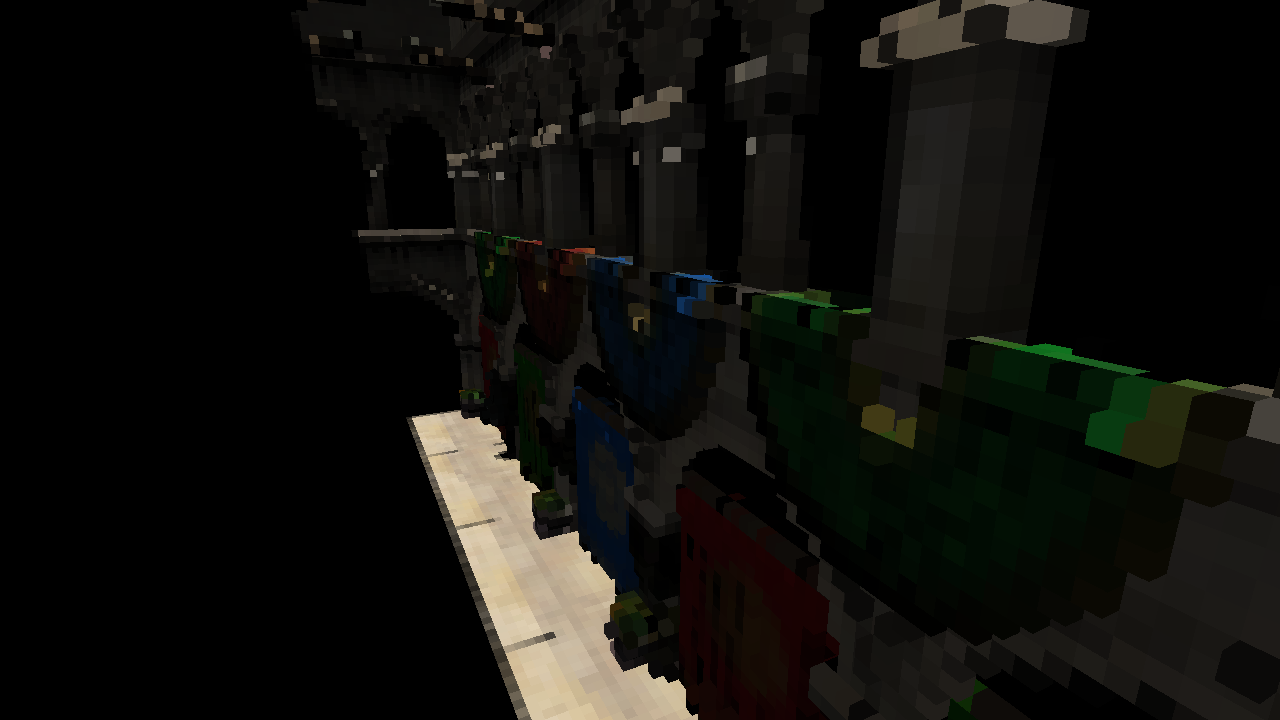
\includegraphics[width=\linewidth]{media/voxel_direct.png}
	\end{subfigure}%
	\hspace{0.01\textwidth}
	\begin{subfigure}[t]{0.49\textwidth}
		\centering
		\captionsetup{justification=centering}
		\caption*{Con iluminación indirecta.}
		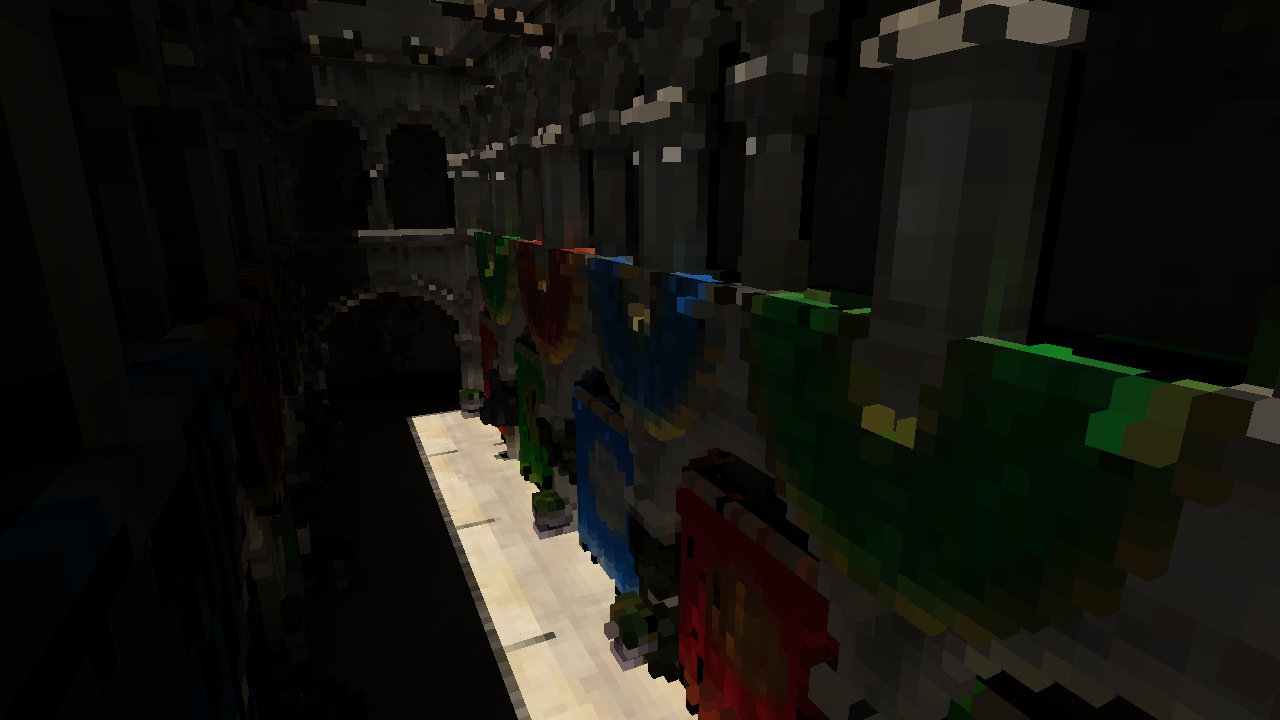
\includegraphics[width=\linewidth]{media/voxel_gi.png}
	\end{subfigure}%
	\par\smallskip
	\begin{subfigure}[t]{0.49\textwidth}
		\centering
		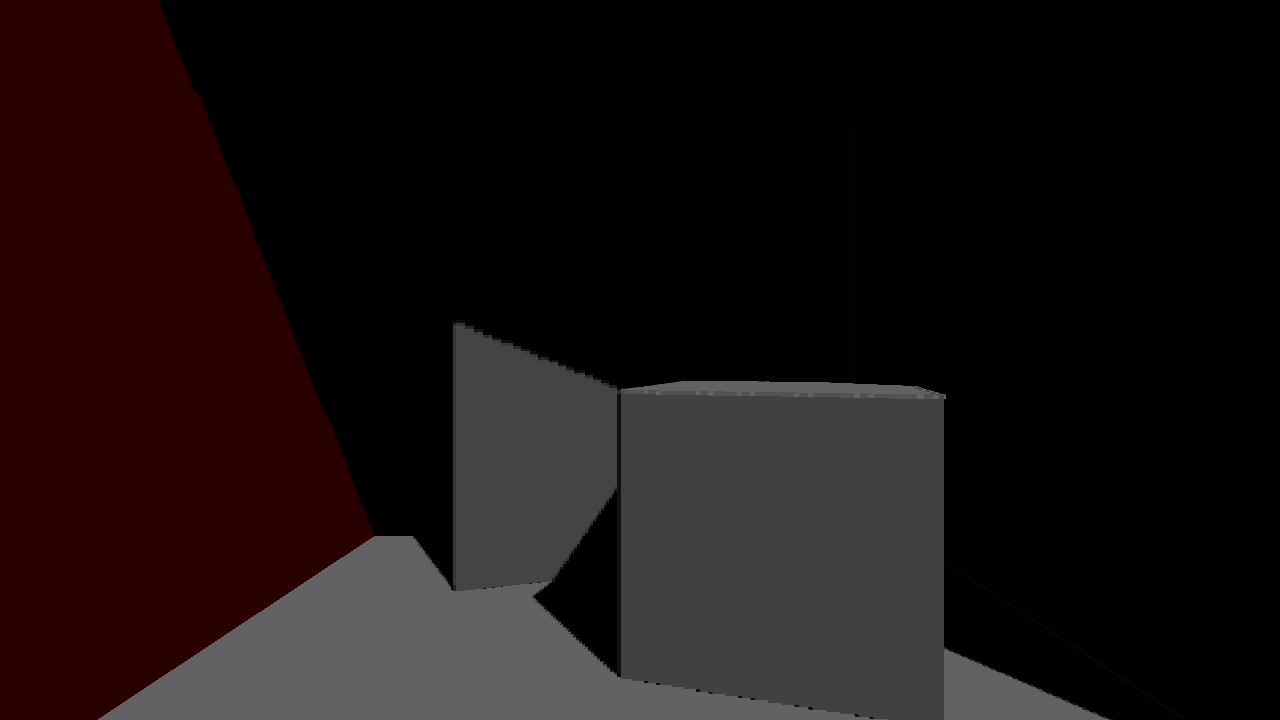
\includegraphics[width=\linewidth]{media/c_voxel_direct.png}
	\end{subfigure}%
	\hspace{0.01\textwidth}
	\begin{subfigure}[t]{0.49\textwidth}
		\centering
		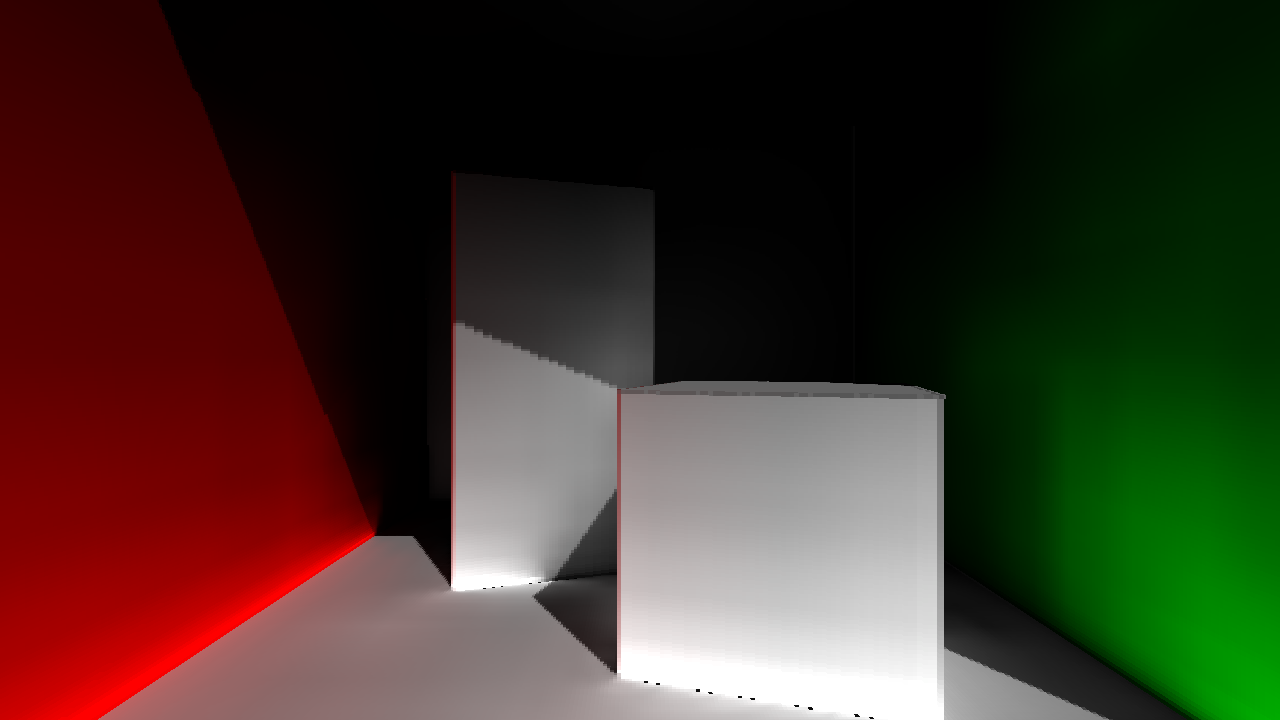
\includegraphics[width=\linewidth]{media/c_voxel_gi.png}
	\end{subfigure}%
	\caption{Resultado de vóxeles con solo iluminación directa y con iluminación global difusa.}
	\label{fig:vgi_scenes}
\end{figure}
% section iluminacion_global_de_voxeles (end)
